%AMB Y processing diagram

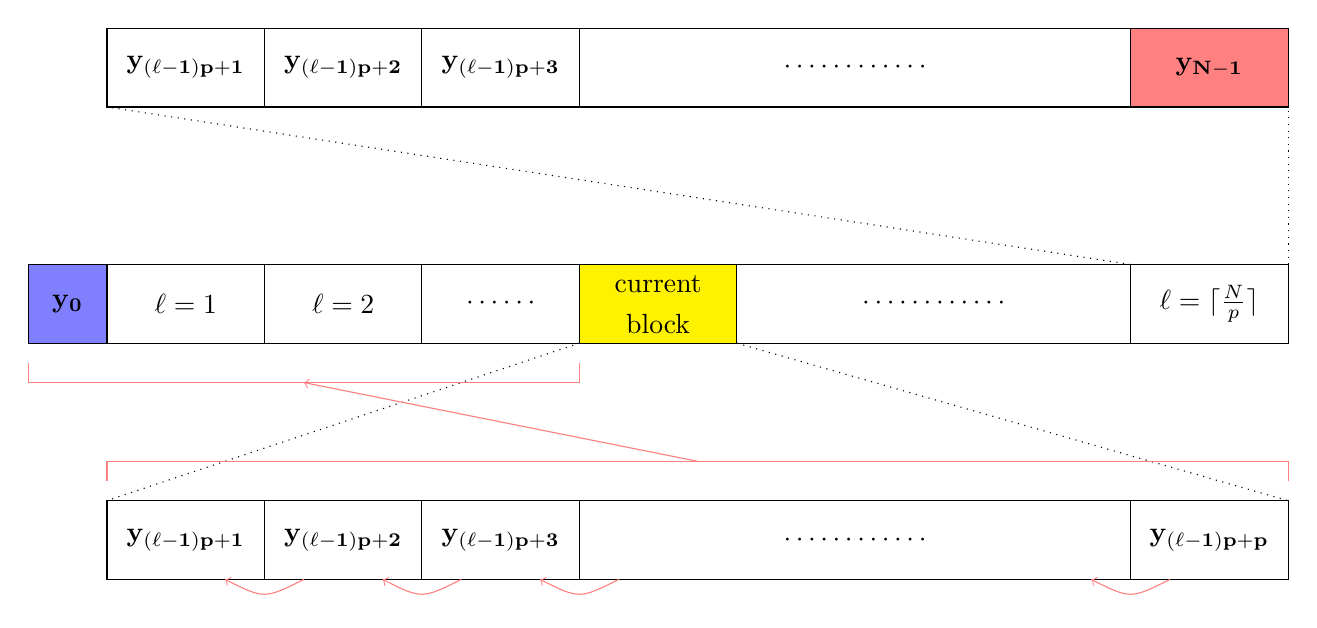
\begin{tikzpicture}
    \filldraw[fill=blue!50] (-1,0) rectangle (0,1);
    \draw (0,0) -- (0,1);
    \draw (-0.5,0.5) node { $ \mathbf{y_0} $ };
    \draw (-1,0) -- (15,0) -- (15, 1) -- (-1, 1) -- cycle;
    \draw (2,0) -- (2,1);
    \draw (4,0) -- (4,1);
    \draw (1,0.5) node { $ \ell = 1 $ };
    \draw (3,0.5) node { $ \ell = 2 $ };
    \draw (5,0.5) node { $ \cdots \cdots $ };
    \draw (6,0) -- (6,1);
    \draw (8,0) -- (8,1);
    \draw (10.5,0.5) node { $ \cdots \cdots \cdots \cdots  $ };
    \draw (13,0) -- (13,1);
    \draw (14,0.5) node { $ \ell = \lceil \frac{N}{p} \rceil $ };
    \filldraw[fill=yellow] (6,0) rectangle (8,1);
    \draw (7,0.75) node { current };
    \draw (7,0.25) node { block };
    \draw [dotted] (6,0) -- (0,-2);
    \draw [dotted] (8,0) -- (15,-2);
    \draw (0,-2) -- (15,-2) -- (15,-3) -- (0,-3) -- cycle;
    \draw (2,-3) -- (2,-2);
    \draw (4,-3) -- (4,-2);
    \draw (6,-3) -- (6,-2);
    \draw (13,-3) -- (13,-2);
    \draw (1,-2.5) node { $ \mathbf{ y_{(\ell - 1) p + 1} } $ };
    \draw (3,-2.5) node { $ \mathbf{ y_{(\ell - 1) p + 2} } $ };
    \draw (5,-2.5) node { $ \mathbf{ y_{(\ell - 1) p + 3} } $ };
    \draw (9.5, -2.5) node { $ \cdots \cdots \cdots \cdots $ };
    \draw (14,-2.5) node { $ \mathbf{ y_{(\ell - 1) p + p} } $ };
    \draw [dotted] (13,1) -- (0,3);
    \draw [dotted] (15,1) -- (15,3);
    \draw (0,3) -- (15,3) -- (15,4) -- (0,4) -- cycle;
    \draw (2,3) -- (2,4);
    \draw (4,3) -- (4,4);
    \draw (6,3) -- (6,4);
    \filldraw[fill=red!50] (13,3) rectangle (15,4);
    \draw (13,3) -- (13,4);
    \draw (1,3.5) node { $ \mathbf{ y_{(\ell-1)p + 1} } $ };
    \draw (3,3.5) node { $ \mathbf{ y_{(\ell-1)p + 2} } $ };
    \draw (5,3.5) node { $ \mathbf{ y_{(\ell-1)p + 3} } $ };
    \draw (9.5,3.5) node { $ \cdots \cdots \cdots \cdots $ };
    \draw (14,3.5) node { $ \mathbf{ y_{N-1} } $ };
    \draw [color=red!50, arrows={->}] (13.5,-3) .. controls (13,-3.25) .. (12.5,-3); 
    \draw [color=red!50, arrows={->}] (6.5,-3) .. controls (6,-3.25) .. (5.5,-3); 
    \draw [color=red!50, arrows={->}] (4.5,-3) .. controls (4,-3.25) .. (3.5,-3);    
    \draw [color=red!50, arrows={->}] (2.5,-3) .. controls (2,-3.25) .. (1.5,-3);
    \draw [color=red!50] (-1,-0.25) -- (-1,-0.5) -- (6,-0.5) -- (6,-0.25);
    \draw [color=red!50] (0,-1.75) -- (0,-1.5) -- (15,-1.5) -- (15,-1.75);
    \draw [color=red!50, arrows={->}] (7.5,-1.5) -- (2.5, -0.5);
\end{tikzpicture}
